\documentclass{standalone}
\usepackage{tikz} % http://ctan.org/pkg/pgf
\usetikzlibrary{spy, backgrounds}

\begin{document}

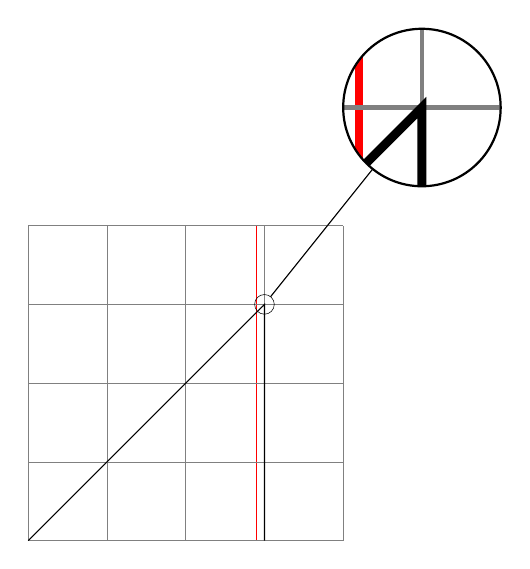
\begin{tikzpicture} [spy using outlines={circle, magnification=8, size=2cm, connect spies, transform shape}]
	\draw[red] (2.9,0) -- (2.9,4);
	\draw[help lines] (0,0) grid (4,4);
	\draw (0,0) -- (3,3) -- (3,0);
	%   \begin{pgfonlayer}{background}
	%    \draw[red] (2.9,0) -- (2.9,4);
	%   \end{pgfonlayer}
	\spy [black] on (3,3) in node [left] at (6,5.5);
\end{tikzpicture}
\end{document}